\subsection*{NSC in the retina and visual cortex}

Due to its roots in efficient-coding theories of natural image processing,
\ac{NSC} figures prominently in the vision neuroscience literature.

For example, \ac{NMF}-based models were able to reconstruct
\emph{in vitro} neuronal spike trains from the salamander retina 
\cite{Onken2016,Liu2017}.
By combining spike-triggered average with \ac{NMF},
Liu and colleagues \cite{Liu2017} were able to identify the subunit layout
of retinal ganglion cells
(Fig.~\ref{fig:NMF|retina}).
Whereas modules were constrained to have nonnegative elements,
stimuli were represented by their contrast values (i.e., their relative deviation from mean light intensity, which could be positive or negative).
The goal of their \ac{NMF} variant was then to seek weights and nonnegative modules
that minimize the difference, in a least-squares sense, between the spike-triggered
stimuli and the reconstruction.
Interestingly, the identified subunits corresponded to 
individual presynaptic bipolar cells,
as verified by multielectrode array recordings with simultaneous recordings from
individual bipolar cells through sharp microelectrodes \cite{Liu2017}.
This allowed the researchers to improve predictions about how ganglion cells respond
to natural stimuli, without the need to guess a specific model structure that may be constrained in terms of the size, shape, number, or nonlinearity of 
ganglion cell subunits.
\mikeNote{R1: Fig.5, provide a succinct summary or schematic of STNMF. Also, panel A is not very clear to me (although I haven’t looked at the source paper). Panel B: are the subunits and the modules the same?}

\begin{figure}[ht]
	\centering
	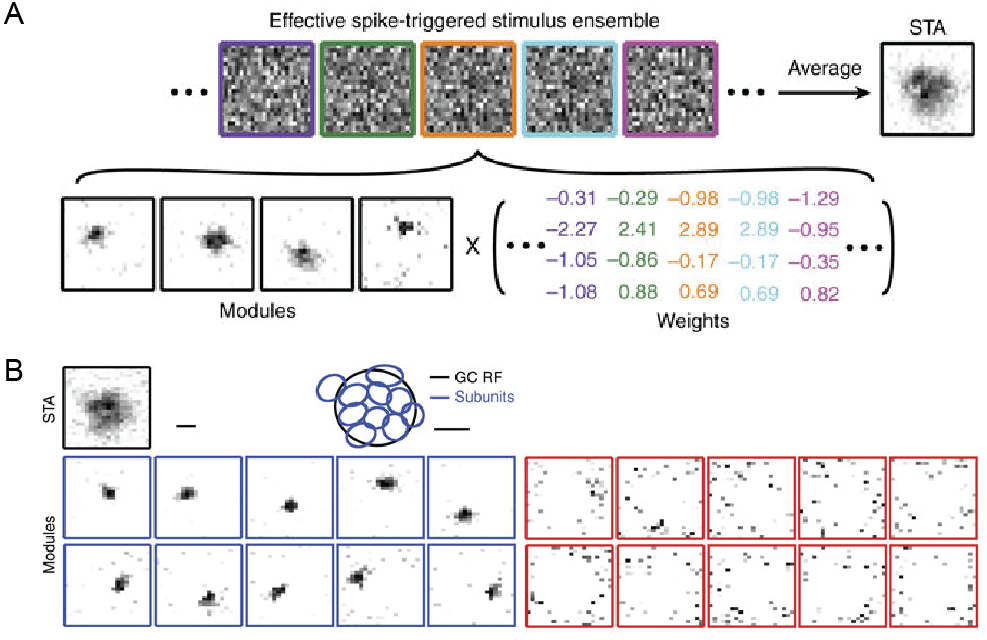
\includegraphics[width=\textwidth]{fig-rev1-retina}
    \caption{
    Identification of retinal ganglion cell subunits 
    with \ac{STNMF} (adapted \revise{with permission} from \cite{Liu2017}).
    \textbf{\emph{A}},
	     Samples of a ganglion cell’s effective spike-triggered stimulus ensemble (top),
         whose average corresponds to the cell’s \ac{STA}.
         For easier visual comparison with the subunits,
         \acp{STA} are displayed with negative pixel values set to zero and
         with zero corresponding to white in the grayscale image.
         \ac{STNMF} decomposes this ensemble into a set of modules and 
         a weight matrix (bottom).
         The example here shows four modules that were identified for
         a sample ganglion cell.
    \textbf{\emph{B}},
         Modules obtained for another sample ganglion cell by applying \ac{STNMF}
         with 20 modules (bottom 2 rows). Some modules have a strongly localized structure 
         (blue frames), others are more noise-like (red frames).
         The top row shows the cell’s receptive field,
         given by the spatial component of the STA, as well as the fitted \ac{RF} outline
         (GC RF, black ellipse), together with outlines of the localized subunits 
         (blue ellipses). Scale bars, 100 µm.
    }
	\label{fig:NMF|retina}
\end{figure}

As mentioned in the previous section,
\ac{NSC} has been extensively applied to early visual cortex,
where it has successfully explained 
orientation and frequency tuning of simple and complex cells in \ac{V1} \cite{Hoyer2003},
edge-like pooling of spatial frequency channels in V2 \cite{Hyvarinen2005},
including \ac{RF} properties such as end-stopping and contour integration 
\cite{HoyerHyvarinen2002}.
With the exception of face processing in \ac{IT}
\cite{LeeSeung1999,ChangTsao2017},
\ac{NSC} has yet to be applied to higher-order areas in the ventral visual stream.
The success of \ac{NSC} in explaining V1 and V2 response properties
suggests that it might be possible to extend the model to texture integration in
V4.

In our own work, we found evidence for \ac{NSC} in the dorsal visual stream.
Specifically, we demonstrated that simulated neurons 
in a \ac{NSC} based model of \ac{MSTd} 
responded to  large optic flow fields in much the same way as real neurons in macaque \ac{MSTd} \cite{Beyeler2016}.
Fig.~\ref{fig:NMF|MSTd} shows the distribution of direction preferences
of \ac{MSTd} cells (Fig.~\ref{fig:NMF|MSTd}A, B; \cite{Takahashi2007})
and \ac{MSTd}-like model units (Fig.~\ref{fig:NMF|MSTd}C, D; \cite{Beyeler2016})
for \revise{rotation and translation, respectively}.
Each data point in the scatter plots specifies the preferred 3D direction
of a single neuron or model unit.
Histograms along the boundaries show the marginal distributions of azimuth
and elevation preferences.
Not only did individual units match response properties of individual neurons
in macaque \ac{MSTd},
but the model was able to recover statistical properties of the \ac{MSTd}
population as a whole, such as a relative overrepresentation of lateral
headings (Fig.~\ref{fig:NMF|MSTd}C, D).

\begin{figure}[ht]
	\centering
	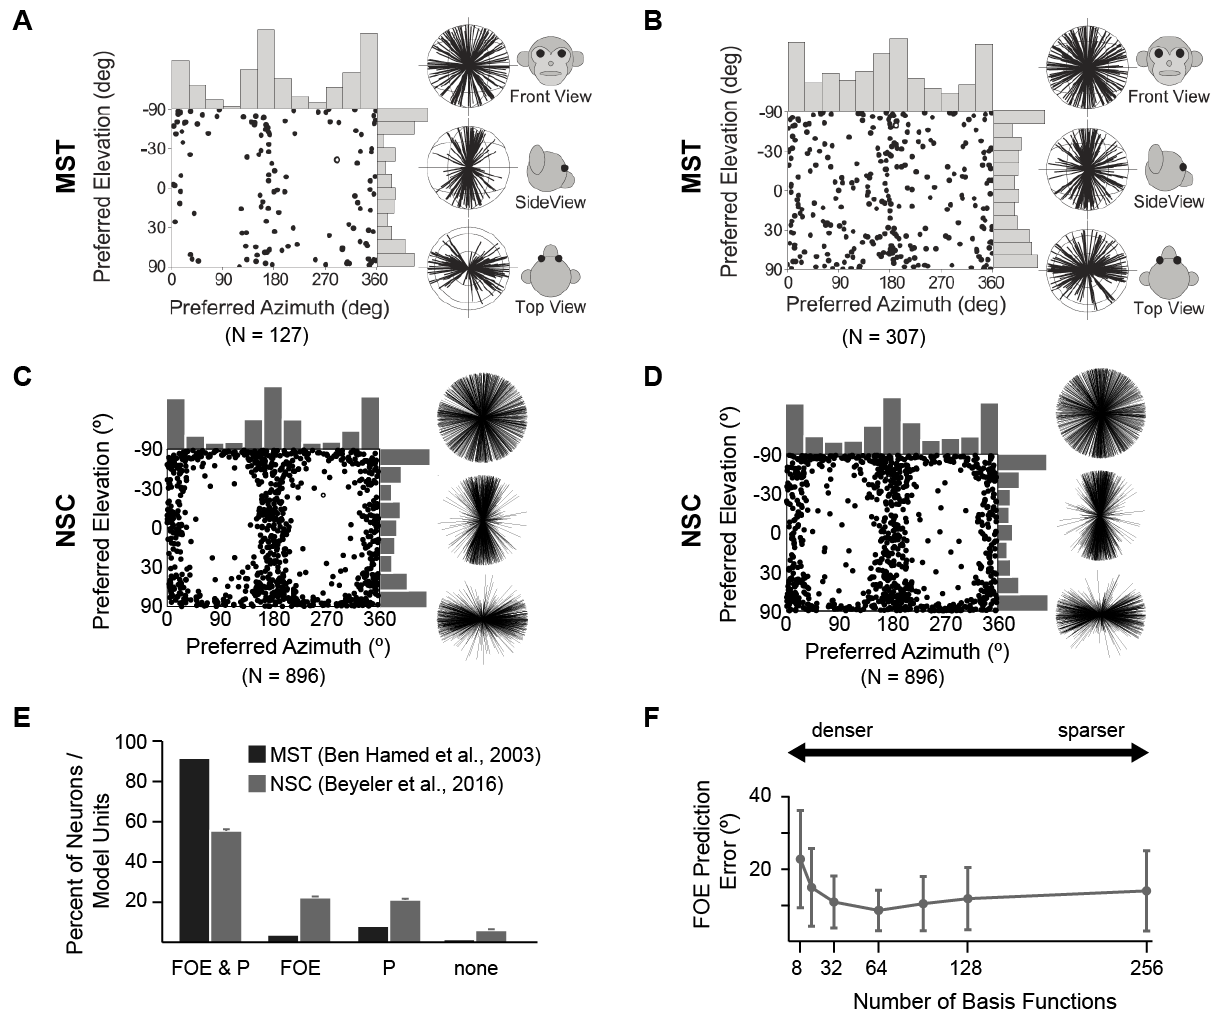
\includegraphics[width=0.95\textwidth]{fig-rev1-MST}
    \caption{
    \textbf{\emph{A-D}},
         Distribution of 3D direction preferences of macaque \ac{MSTd} neurons
         (rotation, \textbf{\emph{A}}; translation, \textbf{\emph{B}}; 
         reprinted \revise{with permission} from \cite{Takahashi2007})
         and model units in the \ac{NSC}-based sparse decomposition model
         (rotation, \textbf{\emph{C}}; translation, \textbf{\emph{D}}; 
         reprinted \revise{with permission} from \cite{Beyeler2016}).
         Each data point in the scatter plots corresponds to the preferred azimuth
         (abscissa) and elevation (ordinate) of a single neuron.
         Histograms along the top and right sides of each scatter plot show the
         marginal distributions.
         Also shown are 2D projections (front view, side view, and top view)
         of unit-length 3D preferred direction vectors (each radial line represents
         one neuron).
    \textbf{\emph{E}},
         Distribution of focus of expansion (FOE) and pursuit (P) selectivities
         in macaque \ac{MSTd} (dark gray) and model \ac{MSTd} (light gray;
         reprinted \revise{with permission} from \cite{Beyeler2016}).
         Neurons or model units were involved in encoding heading (FOE),
         eye velocity (P), both (FOE \& P), or neither (none).
    \textbf{\emph{F}},
         Heading prediction (generalization) error as a function of the
         number of basis functions using cross-validation.
         Vertical bars are the SD (reprinted \revise{with permission}
         from \cite{Beyeler2016}).
    }
	\label{fig:NMF|MSTd}
\end{figure}

\ac{MSTd} is known to encode a number of perceptual variables,
such as the direction of travel (heading) and eye rotation velocity.
During forward movement, retinal flow radiates out symmetrically from a single point,
the focus of expansion (FOE), from which heading can be inferred.
However, instead of consisting of a set of distinct subpopulations,
each specialized to encode a particular perceptual variable,
\ac{MSTd} has been found to consist of neurons that act more like basis functions,
where a majority of cells were involved in the simultaneous encoding of multiple
perceptual variables (Fig.~\ref{fig:NMF|MSTd}E).
A similar picture emerged when we investigated the involvement of \ac{MSTd}-like
model units in the encoding of both heading and eye rotation velocity
(Fig.~\ref{fig:NMF|MSTd}E).

Interestingly, the sparsity regime in which model \ac{MSTd} achieved the
\mikeNote{One reason why remapping into a different basis makes sense is that it might be easier to read out certain variables. For example, reading out heading in the MSTd basis is supposedly easier than in the MT basis. A similar thing might be true for RSC. Need to make this point stronger for R2 - possibly in the Discussion, too.}
lowest heading prediction error (Fig.~\ref{fig:NMF|MSTd}F) was also the
regime in which \ac{MSTd}-like model units reproduced a variety of known
\ac{MSTd} visual response properties
(for experimental details refer to \cite{Beyeler2016}).
In contrast to findings about early visual cortex,
this regime does not use an overcomplete basis set \cite{OlshausenField1996},
yet can still be considered a sparse coding regime \cite{SpanneJorntell2015}.
Such an intermediary sparse code might be better suited
(as opposed to an overcomplete basis set)
for areas such as \ac{MSTd},
because the increased memory capacity of such a code might lead to compact
and multifaceted encodings of various perceptual variables
\cite{BenHamed2003}.


\subsection*{NSC in the auditory cortex}

The auditory cortex is a prime example of efficient coding. The auditory system is believed to decompose auditory signals into
a set of elementary acoustic features \cite{SmithLewicki2006},
such that the complete acoustic waveform can be described by a
sparse population code that operates near an information-theoretic optimum
\cite{SmithLewicki2006,rokem2006,Hromadka2008}.
It is therefore not surprising that computational models based on \ac{NSC}
have been very successful at describing the spectro-temporal \acp{RF}
of neurons in the \ac{A1} \cite{Martinez2015,David2007}.
Response properties of \ac{A1} neurons are well described by a spectrogram;
they are often tuned to stimulus frequency but are rarely phase-locked
to oscillations of the sound waveform \cite{Leaver2010}.
The cortical representation of auditory signals seems to not only be sparse,
but also rely on statistically independent acoustic features \cite{Klein2003}.

Similar to visual cortex, auditory cortex is hierarchically organized,
with neurons in \ac{A1} responding to simple acoustic features of natural sounds,
and higher-order areas responding to more behaviorally relevant stimuli.
The anterior superior temporal region of auditory cortex, for example,
responds to categories of acoustic objects,
such as sounds produced by voices and musical instruments
\cite{Leaver2010}.
An intriguing question for future modeling studies is therefore 
whether \ac{NSC} can be extended to the next level of the auditory hierarchy:
Would it be possible to construct more complex acoustic objects from a sparse,
parts-based set of elementary, \ac{A1}-like acoustic features?
And would the representation of such acoustic objects resemble neuronal responses
in the anterior superior temporal region of auditory cortex?


\subsection*{NSC in the olfactory cortex}

In contrast to most other sensory modalities, 
the basic perceptual dimensions of olfaction remain unclear.
Odors evoke complex responses in granule cells (located in the olfactory bulb)
that evolve over hundreds of milliseconds \cite{Broome2006}.
Granule cells use a sparse combinatorial code to convey information about odor identity
and concentration \cite{Koulakov2011,Gupta2015}.
Downstream from the olfactory bulb, odors tend to activate a small but consistent
proportion ($\sim 10\%$) of cortical neurons in the piriform cortex \cite{poo2009},
which is thought to form odor object percepts \cite{chen2014,stettler2009}.
Although piriform cortex is not topographically organized,
a spatial structure can be discerned when examining the projections of output neurons,
which are highly segregated and functionally specific.
Whereas the anterior piriform cortex is associated with the encoding of 
odor identity and odor structure, 
the posterior piriform cortex is involved in associational aspects of odors, 
such as valence and similarity \cite{chen2014,gottfried2006}.

Castro and colleagues \cite{Castro2013} provided 
one of the most compelling pieces of evidence for \ac{NSC}
in the olfactory system to date:
In an effort to elucidate the dimensions along which perceptual space might be
organized in the olfactory system,
they applied \ac{NMF} to a dataset of 144 monomolecular odors,
each represented by a 146-dimensional odor profile.
Each dimension in the odor profile corresponded to the rated applicability of
a number of semantic labels, such as `sweet', `floral', and `heavy'
(Fig.~\ref{fig:evidence-olfaction}A).
By applying \ac{NMF} to the odor profile, they showed that a small, sparsely active set of basis functions could accurately describe any odor in the dataset
(Fig.~\ref{fig:evidence-olfaction}C).
Interestingly, \ac{NMF} revealed a prominent block
diagonal structure to the full matrix \textbf{H}
(Fig.~\ref{fig:evidence-olfaction}B), indicating that:
1) a given odor tended to be characterized by a single prominent dimension,
implying that the basis functions recovered by \ac{NMF} were perceptually meaningful,
and 2) all 10 dimensions were occupied,
implying that the basis functions recovered by \ac{NMF} could span the space of
behaviorally relevant odors.
This suggests that a given odor percept may be considered an 
instance of one of several fundamental qualities.
For the data set investigated, individual odor profiles were well-classified 
by their proximity to a single one of these dimensions, 
with all ten dimensions being approximately equally expressed 
across the set of odors.
\mikeNote{R1: Fig 7: I’m a bit confused about the nomenclature in the figure, its caption and the text. Please revise}

\begin{figure}[ht]
	\centering
	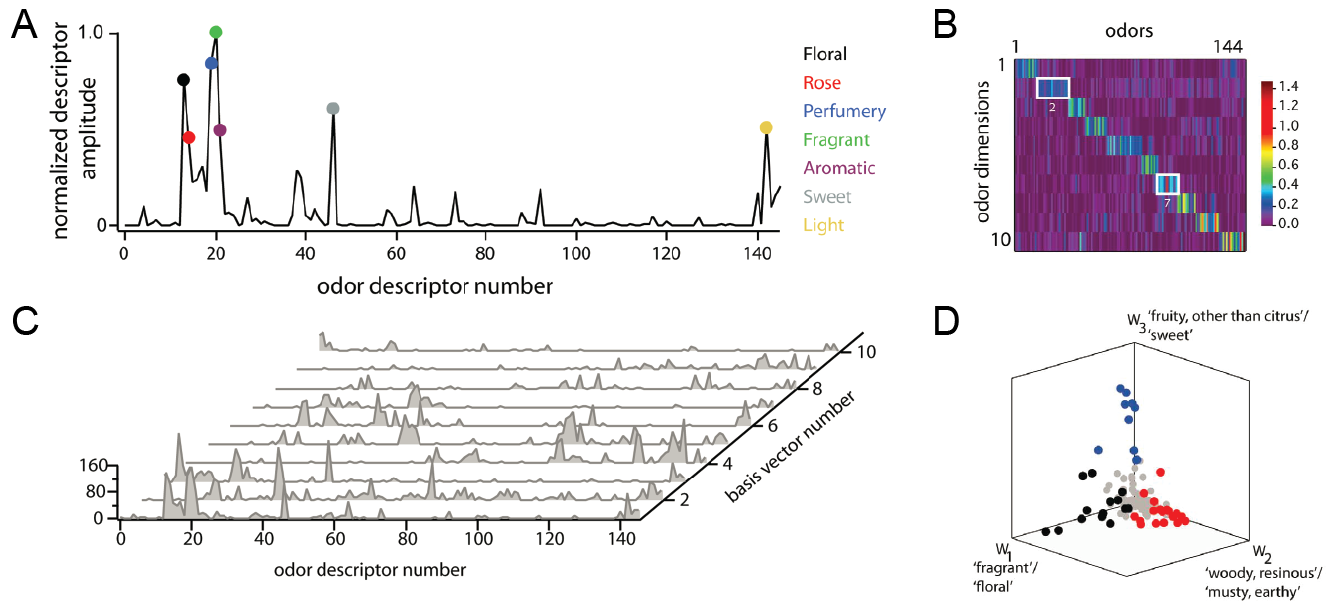
\includegraphics[width=\textwidth]{fig-rev1-olfaction}
    \caption{\ac{NMF} recovers a sparse and parts-based representation
    of olfactory perceptual space (reprinted \revise{with permission} 
    from \cite{Castro2013}).
       \textbf{\emph{A}},
          Plot of normalized odor descriptor amplitude vs. odor descriptor number for
          the first basis function. Each point along the x-axis corresponds to a single
          odor descriptor, and the amplitude of each descriptor indicates the
          descriptor's relevance to the shown perceptual basis function.
          Colored circles show the 7 largest elements, with corresponding descriptors
          listed on the right.
       \textbf{\emph{B}},
          Waterfall plot of the 10 basis functions constituting \textbf{W}.
       \textbf{\emph{C}},
          Heat map of the coefficient matrix, \textbf{H},
          where each column of \textbf{H} corresponds to a different odor.
          Columns of \textbf{H} are normalized and sorted into groups defined by
          peak coordinate (1-10).
       \textbf{\emph{D}},
          Plot of all 144 odors in the dataset (each point is a column in \textbf{H})
          in the space spanned by the first three basis functions.
          Black, red, and blue points are those with peak coordinates in dimensions
          1, 2, and 3, respectively. Gray points are all remaining odors.}
	\label{fig:evidence-olfaction}
\end{figure}

Furthermore, \ac{NMF} recovered basis functions whose descriptors align
with perceptual dimensions highlighted in several previous analyses of odor space,
including but not limited to relative pleasantness (e.g., `fragrant`, `sickening`), 
and potential palatability (`woody, resinous', `chemical', `sweet', and `lemon').
Odors clustered predominantly along these axes
(Fig.~\ref{fig:evidence-olfaction}D), 
motivating the interpretation that odor space is organized 
by a relatively large number of independent qualities that apply categorically
\cite{Castro2013}.


\subsection*{NSC in the somatosensory cortex}

Of all of the sensory areas,
\mikeNote{R1: Most of the studies that the authors discuss are from the mouse barrel. However, these results may not generalize to primates: for example, London \& Miller showed that neurons in the proprioceptive arm area of S1 respond to movements in many directions [11], which seems at odds with the results for the barrel cortex. Also, my concerns about the homunculus in M1 also apply to S1. I’d also suggest the authors to revise some primate studies in touch, e.g., by the Bensmaia lab, to expand this section.}
somatosensory cortex is among the best understood in terms of circuitry,
yet least understood in terms of sensory function
\cite{Ramirez2014}.
Spatiotemporal receptive fields indicate that individual neurons respond to a small number of stimulus dimensions, suggesting a role for dimensionality reduction in primary somatosensory cortex \cite{Ramirez2014}.
In an effort to elucidate the stimulus dimensions that individual neurons respond to,
Whiteway and Butts \cite{WhitewayButts2017} devised the \ac{RLVM},
a combination of nonlinear dimensionality reduction with nonnegativity constraints
that is closely related to \ac{NSC}.
When they applied the \ac{RLVM} to 
a two-photon imaging dataset of hundreds of simultaneously recorded neurons 
in mouse primary somatosensory cortex while the animal was performing
a tactile discrimination task,
they found basis functions that properly identified individual neurons.
Similar to the recorded neuronal responses, these basis functions were closely related
to both the tactile stimulation as well as 
nonstimulus aspects of the behavioral task.
Furthermore, \ac{RLVM} achieved a lower reconstruction error than other
linear dimensionality reduction techniques such as \textbf{\ac{PCA}}.

Similar to auditory cortex,
activity in somatosensory cortex can be extremely sparse
\cite{Jadhav2009,oconnor2010,Crochet2011},
and sparse coding models have successfully explained the response properties
of individual neurons in rat somatosensory cortex (e.g., \cite{Hafner2004}).
In addition, the presence of a topographically organized sensory `homunculus' 
in various species \cite{penfield1937,hari1993,petersen2007} 
suggests a possible parts-based representation scheme.


\subsection*{NSC in the retrosplenial cortex (RSC)}

In our own work, we found evidence that \ac{NSC} 
can explain response properties in \ac{RSC}, 
an area important for navigation and spatial memory 
\cite{Miller2014,Nelson2015,VannAggleton2009}.
Using a similar methodology to \cite{Beyeler2016},
we applied \ac{NMF}, with a sparsity constraint,
to parameterized behavioral variables extracted from electrophyisiological recordings
of \ac{RSC} neurons in the rat \cite{AlexanderNitz2015}
while the animal ran back and forth a W-shaped track
(for experimental details, see Supplementary Material).
As mentioned above, these behavioral variables included the animal's position, head direction, 
and movement direction (Fig.~\ref{fig:NMF|reconstruction}C).
The basis functions recovered by \ac{NMF} were then used to generate simulated responses
of model \ac{RSC} neurons according to Eq.~\ref{eqn:nsc-model-response},
and the simulated responses were compared to neuronal responses 
from the electrophysiological recordings.

We found that the population activity of these simulated neurons could be used to predict
the animal's location both with respect to the beginning of the route
(route-based reference frame)
and with respect to where the route was located within the room
(allocentric reference frame).
In addition, simulated neuronal activity could be classified into three broad categories,
with remarkably similar population statistics to rat \ac{RSC}:
1) responding to left and right turns on a specific position along the route,
2) responding to left and right turns regardless the position along the route,
and 3) exhibiting complex and robust firing patterns without turn sensitivity
(see Supplementary Material; also Fig.~\ref{fig:NMF|RSC}A, B).


\subsection*{Reinforcement-driven NSC in the basal ganglia}

\mikeNote{R1: To reach a broader audience, the authors should describe better the mechanisms of Hebbian and Anti-Hebbian plasticity in the Basal ganglia section.}
There is computational evidence 
for a reward-driven variant of \ac{NSC} in the basal ganglia, 
a cluster of deep forebrain nuclei that are involved in the 
processing of motor, associative, and limbic information
(for recent reviews see \cite{BarGad2003_Review,NelsonKreitzer2014}).
The basal ganglia connect most cortical areas to the frontal cortex through
a series of convergent and sparsely connected pathways \cite{schwab2015},
where signals from tens of millions of cortical neurons are projected
onto a $10 - 10,000$ fold smaller population of neurons in different subnuclei
of the basal ganglia \cite{BarGad2003_Review}.

The \ac{RDDR} model suggests that dimensionality reduction 
in the cortico-basal ganglia pathway is achieved via
a combination of Hebbian and anti-Hebbian learning rules
that are implemented by feedforward excitatory and lateral inhibitory
connections \cite{BarGad2000,BarGad2003_Review}. \revise{These learning rules control the strength of synaptic weights in the network by altering a given weight in proportion to the correlation between the firing rates of the input and output neurons. In Hebbian learning, synaptic weights are strengthened given a positive correlation (a phenomenon referred to as long-term potentiation, or LTP), while synaptic weights are depressed if the firing rate correlation is negative (referred to as long-term depression, or LTD). In order to implement dopamine-modulated Hebbian learning in this model, a reinforcement signal was used to dictate the level of dopamine in the circuit (1 for reward-related events, 0 for background levels of dopamine when reward-related events or information are not present, and negative values to simulate dopamine depeletion \cite{BarGad2000}). The value of the reinforcement signal determined how much learning was allowed to occur.}

In the \ac{RDDR} model, a reinforcement signal corresponding to dopamine modulates the Hebbian learning rule 
of the feedforward projections,
allowing the network to learn to extract input dimensions
that are associated with reward activity
while suppressing behaviorally irrelevant input dimensions.
Whereas the original \ac{RDDR} model was a neural-network based model
for performing \ac{PCA} \cite{BarGad2000},
later iterations incorporated nonnegativity constraints on the
connection weights that effectively transformed the model 
into an \ac{NMF} variant \cite{BarGad2003_Review}.

In addition to suggesting a role for lateral connectivity
in the basal ganglia,
the \ac{RDDR} model also advanced understanding of basal ganglia dysfunction
in movement-related disorders such as Parkinon's and Huntington's disease. \revise{Previous studies have indicated that when the basal ganglia is functioning normally and is then subjected to focal lesions, these lesions have minimal impact on behavior. Bar-Gad and colleagues \cite{BarGad2000}
suggested that this is an expected finding because of the network's ability to reorganize connections,
whereas abnormal dopamine levels should significantly alter 
the reinforcement signal that controls the model's ability 
to discriminate behaviorally relevant input signals (as in Parkinson's disease). Accordingly, restoration of background dopamine levels via dopamine replacement therapy alleviate the symptoms, consistent with results of dopamine depletion and restoration in the model.}
\mikeNote{R1: cliffhanger: Did Bergman and colleagues test their predictions for focal lesions? What would the authors expect?}
\emilyNote{clarified that this was a post-hoc explanation of their model and added actual predictions.}

\revise{The RDDR model made two critical predictions, one of which has yet to be tested experimentally. First, this model was initially developed to explain the existence of the extensive inhibitory lateral connectivity found within the basal ganglia, which seem to have no functional purpose based on experimental data\emilyNote{clunky sentence, revise}. The RDDR model predicts that these connections facilitate learning and must thus be studied during the learning phase of a task either in young animals or in animals being exposed to a new environment. At this time, the lateral connections should show increased strength and the firing patterns of the connected neurons should be correlated. After learning, these connections are expected to rapidly lose efficacy. Second, at the time, Hebbian and anti-Hebbian learning modulated by a dopaminergic reinforcement signal had yet to be documented in the basal ganglia. However, since publication this prediction has been confirmed, as studies have revealed dopamine-modulated LTP and LTD as mechanisms that facilitate learning in corticostriatal synapses \cite{calabresi2007dopamine}.}

\emilyNote{While working on this, I found another Bar-Gad article that talks about somatotopic organization in the BG corresponding to face, arms, legs, etc, which may or may not be useful to bring up re: parts-based coding. https://www.frontiersin.org/articles/10.3389/fnsys.2011.00038/full}

